\documentclass[11pt, a4paper]{article} 

\usepackage[T1]{fontenc}
\usepackage[utf8]{inputenc}
\usepackage[british]{babel}  
\usepackage[left = 0mm, right = 0mm, top = 0mm, bottom = 0mm]{geometry}
\usepackage[stretch = 25, shrink = 25, tracking=true, letterspace=30]{microtype}  
\usepackage{graphicx}
\usepackage{xcolor}
\usepackage{marvosym}

\usepackage{enumitem}
\setlist{parsep = 0pt, topsep = 0pt, partopsep = 1pt, itemsep = 1pt, leftmargin = 6mm}

\usepackage{FiraSans}
\renewcommand{\familydefault}{\sfdefault}

\definecolor{cvblue}{HTML}{304263}

\newcommand{\dates}[1]{\hfill\mbox{\textbf{#1}}}
\newcommand{\is}{\par\vskip.5ex plus .4ex}
\newcommand{\smaller}[1]{{\small$\diamond$\ #1}}
\newcommand{\headleft}[1]{\vspace*{3ex}\textsc{\textbf{#1}}\par%
    \vspace*{-1.5ex}\hrulefill\par\vspace*{0.7ex}}
\newcommand{\headright}[1]{\vspace*{2.5ex}\textsc{\Large\color{cvblue}#1}\par%
     \vspace*{-2ex}{\color{cvblue}\hrulefill}\par}

\usepackage[colorlinks = true, urlcolor = white, linkcolor = white]{hyperref}

\begin{document}

\setlength{\topskip}{0pt}
\setlength{\parindent}{0pt}
\setlength{\parskip}{0pt}
\setlength{\fboxsep}{0pt}
\pagestyle{empty}
\raggedbottom

\begin{minipage}[t]{0.33\textwidth} 
\colorbox{cvblue}{\begin{minipage}[t][5mm][t]{\textwidth}\null\hfill\null\end{minipage}}

\vspace{-.2ex}
\colorbox{cvblue!90}{\color{white}
\kern0.09\textwidth\relax
\begin{minipage}[t][293mm][t]{0.82\textwidth}
\raggedright
\vspace*{2.5ex}

\Large Lisandro \textbf{\textsc{Portaluri López}} \normalsize 

% IMPORTANTE: guardá tu imagen en la misma carpeta que este .tex con el nombre "foto.jpg"
% Si tu archivo tiene otro nombre, cambialo acá abajo
\null\hfill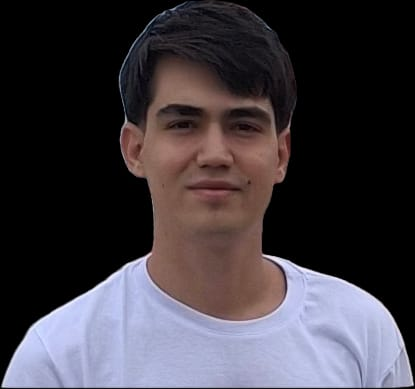
\includegraphics[width=0.65\textwidth]{foto.jpg}\hfill\null

\vspace*{0.5ex}

\headleft{Profile}
Estudiante avanzado y egresado de \textbf{Ingeniería Industrial}, con fuerte orientación a la optimización de procesos y análisis de datos. Me destaco por mi pensamiento analítico, disciplina y capacidad para resolver problemas complejos. Interesado en la mejora continua, la eficiencia operativa y la toma de decisiones basada en datos.

\headleft{Informacion de contacto}
\small
\MVAt\ {lisandroportaluri@gmail.com} \\
\Mobilefone\ +54\,9\,261\,2730309 \\
\Mundus\ \href{https://github.com/lisandro}{github.com/lisandro} \\
\Letter\ Mendoza, Argentina
\normalsize

\headleft{Informacion personal}
Age: \textbf{23} \\
Ciudadania: \textbf{Argentina} \\
Languages: \textbf{Español} (nativo), \textbf{Ingles} (intermedio)


\end{minipage}%
\kern0.09\textwidth\relax
}
\end{minipage}
\hskip2.5em
\begin{minipage}[t]{0.56\textwidth}
\setlength{\parskip}{0.8ex}

\vspace{2ex}

\headright{Experiencia}

\textsc{Asistente de Producción} en \textit{Bodega Andino} \dates{2024--pres.} \\
\smaller{Control de línea de embotellado, optimización de tiempos y reducción de desperdicios.}

\is
\textsc{Analista Junior} en \textit{Metalúrgica Cuyo S.A.} \dates{2023--2024} \\
\smaller{Análisis de costos, mejora de procesos y seguimiento de indicadores (KPIs).}

\is
\textsc{Pasante en Logística} en \textit{Distribuidora Mendoza} \dates{2022--2023} \\
\smaller{Gestión de inventarios, planificación de entregas y uso de Excel para control de datos.}

\headright{Educación}

\textsc{Ingeniería Industrial} \textit{Universidad Nacional de Cuyo} \dates{Egresado} \\
\smaller{Formación en procesos industriales, optimización y gestión.}

\is
\textsc{Educación Secundaria} \textit{Colegio Corazón de María} \dates{} \\
\smaller{Bachiller con orientación en ciencias.}

\headright{Conocimientos y Habilidades}

\textit{Idiomas:} Inglés intermedio (B1) .

\textit{Herramientas computacionales:} Excel avanzado, conocimientos basicos de LaTex y Html.

\textit{Habilidades blandas:} gestion de grupos y proyectos multidiciplinarios (con amplia experiencia).

\end{minipage}

\end{document}
